%% %%%%%%%%%%%%%%%%%%%%%%%%%%%%%%%%%%%%%%%%%%%%%%%%
%% Problem Set/Assignment Template to be used by the
%% Food and Resource Economics Department - IFAS
%% University of Florida's graduates.
%% %%%%%%%%%%%%%%%%%%%%%%%%%%%%%%%%%%%%%%%%%%%%%%%%
%% Version 1.0 - November 2019
%% %%%%%%%%%%%%%%%%%%%%%%%%%%%%%%%%%%%%%%%%%%%%%%%%
%% Ariel Soto-Caro
%%  - asotocaro@ufl.edu
%%  - arielsotocaro@gmail.com
%% %%%%%%%%%%%%%%%%%%%%%%%%%%%%%%%%%%%%%%%%%%%%%%%%

\documentclass[12pt]{article}
\usepackage{design_ASC}
\usepackage{graphicx}
\newcommand{\newpar}{\vspace{0.15in} \noindent}
\usepackage{dcolumn}
\usepackage{fixltx2e}
\DeclareMathOperator{\cov}{cov}
\DeclareMathOperator{\var}{var}

\setlength\parindent{0pt} %% Do not touch this

%% -----------------------------
%% TITLE
%% -----------------------------
\title{Forecasting Consumer Spending in the United States} %% Assignment Title

\author{Sambo Amaza\\ %% Student name
ECON 411 - Economic Forecasting Methods\\ %% Code and course name
\textsc{University of Wisconsin - Milwaukee}
}

\date{May 15, 2020} %% Change "\today" by another date manually
%% -----------------------------
%% -----------------------------

%% %%%%%%%%%%%%%%%%%%%%%%%%%
\begin{document}
\setlength{\droptitle}{-5em}    
%% %%%%%%%%%%%%%%%%%%%%%%%%%
\maketitle
% --------------------------
% Start here
% --------------------------
% %%%%%%%%%%%%%%%%%%%
\section{Introduction}
Consumer spending, also referred to as  personal consumption expenditures (PCE), is the value of the goods and services purchased by, or on the behalf of, U.S. residents. These goods include durable goods (motor vehicles, furnishings and so  on)non durable goods (beverages, clothing), pharmaceutical and other medical products. 
\newpar
\newline
Consumer spending is a key element in economic growth. In the United States, drastic changes consumer spending reflected each time the economy went into recession since 1960. Personal consumption expenditures for durable goods decreased in
all but two of the recessions while personal consumption expenditures for non-durable goods decreased in four of those recessions (McCully). However, previous recessions prior to 1960, experienced real personal consumption expenditures either increasing during the recession or surpassing its previous peak within 18 months of the start of the recession. 
\newpar
\newline
Additionally, consumer spending is an important economic factor because it exhibits a positive relationship with the overall consumer confidence in a nation’s economy. Thus, high levels of  consumer spending is associated with High consumer confidence in the economic market. Consumer confidence provides governments and businesses with an analysis on consumer perception (Vitez). 
\newpar
\newline
The goal of this paper is to use quantitative, statistical/econometric and machine learning methods to studied in ECON 411 (Forecasting Methods) to produce and evaluate consumer spending forecasts.

\section{Data}
This paper makes use of real consumer expenditures (PCE), measured in billions of chained 2012 dollars, in the to forecast the rate of growth in consumer spending. The data set taken into account has a monthly frequency from January 1990 to December 2019 and is seasonally adjusted. As mentioned in the introduction section, consumer confidence is positively related to level of consumer spending and thus, Consumer confidence numbers  from the University of Michigan’s Consumer Sentiment Index (UMCSENT). The period of UMCSENT data included in this project is also from January 1990 to December 2019.
Other data sets included in the estimation and forecast sections because of their predictive ability are the S&P 500 stock prices data sourced from Yahoo! Finance and employment data from the U.S Bureau of Labor Statistics. 

\section{Model Estimation}
In this paper, we make use of a time series model to forecast consumer spending in the United States. The time series forecast equation will take the form of:
\begin{equation} 
\begin{split}
CS_{t+1} & = f(CS_{t},CS_{t-1},CS_{t-2}, CS_{t-3},..., error ) \\
\end{split}
\end{equation}
\newline
where $t$ is the present month, $t+1$ is the next month, $t-1$ is the previous month, $t-2$ is two months ago, and so on. This implies the  prediction of the future consumer spending values in the United States is based on past values of consumer spending itself, but not on external variables which may affect the system. The “error” term in the equation allows for random variation and the effects of relevant variables that are not included in the model.
\newpar
\newline
We make use of the maximum likelihood estimation method to get the best estimates of the above model. First, we make sure that all of the variables in the model are stationary. Thus, we have to check that $y_t$ and all of the predictors for all ($x_{t,1}$,...,$x_{t,k}$) appear to be stationary. Stationarity in our time series data is checked using two unit tests - the Phillip Perron test and the Augmented DIckey-Fuller test. The reports of this test (as reported in the table below) indicate that the data is non-stationary. 
\newpar
\begin{table}[ht]
\centering
\begin{tabular}{r|r|r}
  \hline
 Unit Root Test & ADF & PP \\ 
  \hline
p-value & 0.943 & 0.977 \\
   \hline
\end{tabular}
\caption{ADF and PP Unit Root Tests on real consumer price expenditures}
\end{table}
\newpar
\newpar
\newline
Therefore, we remove the nonstationarity in the data by taking the first difference of the log of the data and retesting for stationarity. The new tests indicate that the growth rate of consumer spending in the United States is now a stationary data. 
\newpar
\newpar
\begin{table}[ht]
\centering
\begin{tabular}{r|r|r}
  \hline
 Unit Root Test & ADF & PP \\ 
  \hline
p-value & 0.02218 & 0.01\\
   \hline
\end{tabular}
\caption{ADF and PP Unit Root Tests on the first lag of real consumer price expenditures}
\end{table}
\newpar
\newline
We can now use a correlogram to determine the appropriate ARMA model in estimating real consumer price expenditures. The Auto correlation Function and Partial Auto Correlation Function plots (see appendix) of the real consumer price expenditures indicate that the most appropriate model in estimating is real consumer price expenditures is a White Noise model.
\newpar
\newline
The White Noise model will serve as a baseline while we generate a vector autoregression (VAR) system, a generalization of the autoregressive model for forecasting a vector of time series. VAR models will allow us to consider a bi-directional relationship with the forecast variable (growth rate of consumer spending) and other predictor variables (employment, S\&P 500 stock prices, consumer sentiment index). Therefore all the variables are modelled as if they influence each other equally. The models are estimated based by equation using the principle of least squares and the goal is to check if the VAR models dominate the white noise process.
\newpar
\newline
The VAR system equations are outlined below:
\newpar

\begin{equation} 
\begin{split}
CS_{t} & = \alpha_t + \beta_1CS_{t-1} + \phi_1EMP_{t-1} + \epsilon_t\\
\end{split}
\end{equation}

\begin{equation} 
\begin{split}
CS_{t} & = \alpha_t + \beta_1CS_{t-1} + \gamma_1CSI_{t-1} + \epsilon_t\\
\end{split}
\end{equation}

\begin{equation} 
\begin{split}
CS_{t} & = \alpha_t + \beta_1CS_{t-1} + \psi_1SP500_{t-1} + \epsilon_t\\
\end{split}
\end{equation}

\begin{equation} 
\begin{split}
CS_{t} & = \alpha_t + \beta_1CS_{t-1} + \phi_1EMP_{t-1} + \psi_1SP500_{t-1} + \epsilon_t\\
\end{split}
\end{equation}

\begin{equation} 
\begin{split}
CS_{t} & = \alpha_t + \beta_1CS_{t-1} + \phi_1EMP_{t-1} + \gamma_1CSI_{t-1}  + \epsilon_t\\
\end{split}
\end{equation}

\begin{equation} 
\begin{split}
CS_{t} & = \alpha_t + \beta_1CS_{t-1} + \psi_1SP500_{t-1} + \gamma_1CSI_{t-1}  + \epsilon_t\\
\end{split}
\end{equation}

\begin{equation} 
\begin{split}
CS_{t} & = \alpha_t + \beta_1CS_{t-1} + \phi_1EMP_{t-1} + \psi_1SP500_{t-1} + \gamma_1CSI_{t-1}  + \epsilon_t\\
\end{split}
\end{equation}
\newpar
\newline
The optimal number of lags for each model stated above will be the model that gives the least selection criteria values. The complete selection criteria values for the first 8 lags are displayed in the Appendix section. However, the optimal lag for each selection criteria is summarized in the table 3 below: 
\newpar
\newpar
\newpar
\newpar
\newpar
\newpar
\newpar
\begin{table}[ht]
\centering
\begin{tabular}{|r|r|r|r|r|}
  \hline
 Model & AIC(n) & HQ(n) & SC(n) & FPE(n) \\ 
  \hline
VAR 1 & 4 & 2 & 1 & 4 \\
 \hline
VAR 2 & 3 & 1 & 1 & 3\\
 \hline
VAR 3 & 4 & 1 & 1 & 4\\
   \hline
VAR 4 & 3 & 1 & 1 & 3\\
   \hline
VAR 5 & 5 & 2 & 1 & 5\\
   \hline
VAR 6 & 2 & 1 & 1 & 2\\
   \hline
VAR 7 & 2 & 1 & 1 & 2\\
   \hline
\end{tabular}
\caption{Model Selection}
\end{table}

The table above indicates some of the selection criteria conflict on some models. For simplicity, we will go with the Schwartz-Bayes Information Criterion (SIC) because it tends to give more parsimonious models that the other selection criteria. Thus, the estimate results for each of the VAR models are displayed in the Appendix section. 

\section{Forecast}
Using an estimation period from January 1990 to December 2017,  a total of 360 observations, as the initial sample estimation to perform out-of-sample forecasting from January 2018 to December, 2019. I use the recursive forecast method to predict 1-step ahead up to 3-step ahead forecasts of Consumer Spending in the United States.
\newpar
\newline
The paper uses the White Noise as a reference model to the more complex VAR models estimated. I calculate the ratio between the root mean squared errors of a VAR model to the AR model in table 2 of the appendix. In the table 3 below, I summarize the superior VAR model at each forecast horizon and provide ratio of the RMSE’s VAR model to the White Noise.
\newpar
\newpar
\newpar
\newpar
\newpar
\begin{table}[ht]
\centering
\begin{tabular}{|r|r|r|r|}
  \hline
Model  & 1-step & 2-step & 3-step \\ 
\hline
\hline
WN &  1.0000 & 1.0000 & 1.0000  \\
\hline
VAR 1 & 1.005451 & 0.9959491 & 1.000131  \\
\hline
VAR 2 & 1.059589 & 1.006045 & 1.000962  \\
\hline
VAR 3 & 0.9820045 & 1.000568 & 1.000568  \\
\hline
VAR 4 & 1.060116 & 0.9964092 & 1.004264  \\
\hline
VAR 5 & 0.9927538 & 0.9956125 & 1.000493  \\
\hline
VAR 6 & 1.053597 & 1.004861 & 1.000926  \\
\hline
VAR 7 & 1.056738 & 0.9970585 & 1.004689  \\
\hline
\end{tabular}
\caption{RMSE results for the forecast horizons}
\end{table}
\newline
Based on the RMSE results above, the VAR 5 model seems to be the model with the lowest root mean squared errors in predicting the 1-step and the 2-step ahead forecasts. The graphs below visually depict how well each of the forecasts models in comparison to actual consumer spending values between January 2017 and December 2019. This plot representation can indicate if there were any data errors and can give an overall idea of the validity of a forecast.
\begin{figure}[!hbt]
     \center
     \caption{Model (4) Forecast vs Actual Growth Rate of Consumer Spending}
     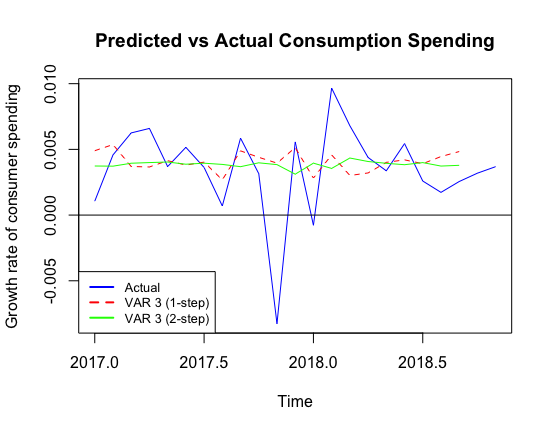
\includegraphics[width=14cm, height=9cm]{forcast pred.png}
\end{figure}
\newpar
\newpar
\newpar
\newpar
\newpar
\newpar
\newpar
\newpar
\newline

Despite the growth rate of consumption spending data being white noise (white noises are difficult to predict because of their random occurrence), the VAR 3 model was able to predict when consumer spending was going to peak and fall. The 1-step ahead, as indicated by the very low RMSE alue in table 4, shows a more accurate forcast of consumer spending growth.

\section{Conclusion}
The forecast results show that the inclusion of the S&P 500 stock prices in a VAR model improves the forecasting of growth rate of consumer spending in the United States. This implies that the bi-variate VAR model with S&P 500 dominates the initial white noise model we had when we plotted the correlogram for the growth rate of consumer spending. 
\newpar
\newline 
Since there is high volatility in growth rate of consumer spending due to its white noise property, further studies should consider including a General Autoregressive Conditional Heteroskedasticity (GARCH) process for a possibility of improving the forecasts made in this paper. The reasoning behind this recommendation is that GARCH processes differ from homoskedastic models, which assume constant volatility, by  depending on past squared observations and past variances to model for current variance. Thus, enhancing the accuracy of ongoing predictions.

\section{References}
McCully, Clinton P. Trends in Consumer Spending and Personal Saving,1959–2009. https:// www.palmislandtraders.com/econ108/psstrend.pdf. Accessed on 04 May 2020.
\newpar
\newline
University of Michigan, University of Michigan: Consumer Sentiment [UMCSENT], retrieved from FRED, Federal Reserve Bank of St. Louis; https://fred.stlouisfed.org/series/UMCSENT, May 9, 2020.
\newpar
\newline
Vitez, Osmond. "The Importance Of Consumer Spending". Smallbusiness.Chron.Com, 2020, https://smallbusiness.chron.com/importance-consumer-spending-3882.html.
\newpar
\newline
U.S. Bureau of Labor Statistics, Employment Level [CE16OV], retrieved from FRED, Federal Reserve Bank of St. Louis; https://fred.stlouisfed.org/series/CE16OV, May 12, 2020
\newpar
\newline
U.S. Bureau of Economic Analysis, Personal Consumption Expenditures [PCE], retrieved from FRED, Federal Reserve Bank of St. Louis; https://fred.stlouisfed.org/series/PCE. May 9, 2020.
\newpar
\newline
Yahoo! Finance, S&P 500 [$^$GSPC], retrieved from Yahoo! Finance; https://finance.yahoo.com. May 9, 2020.

\section{Appendix}

\newpar
\begin{figure}[!hbt]
     \center
     \caption{Real Consumer Spending Expenditures 2010 - 2018}
     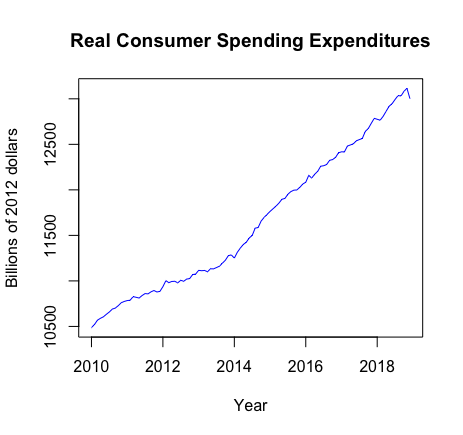
\includegraphics[width=14cm, height=9cm]{rpce.png}
\end{figure}
\begin{figure}[!hbt]
     \center
     \caption{ACF}
     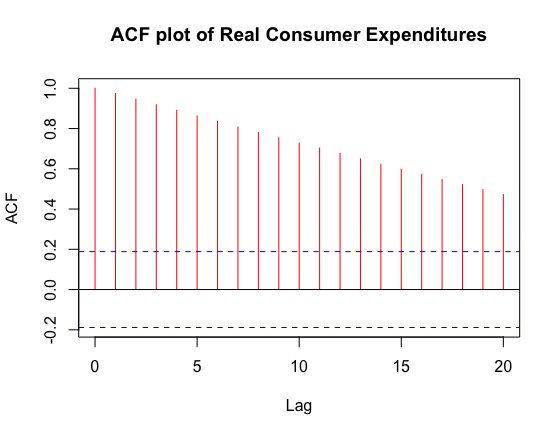
\includegraphics[width=14cm, height=9cm]{acf1.png}
\end{figure}
\begin{figure}[!hbt]
     \center
     \caption{PACF}
     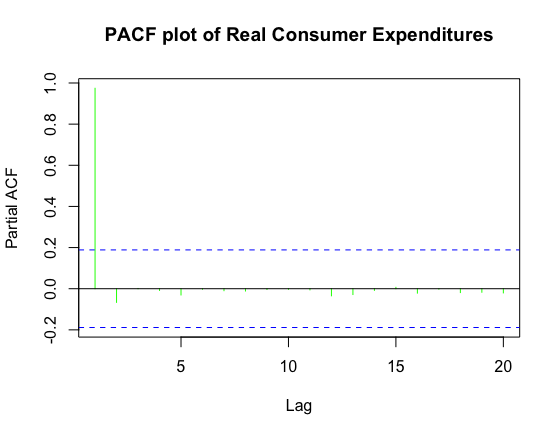
\includegraphics[width=14cm, height=9cm]{pacf1.png}
\end{figure}



\end{document}